\documentclass[1p]{elsarticle_modified}
%\bibliographystyle{elsarticle-num}

%\usepackage[colorlinks]{hyperref}
%\usepackage{abbrmath_seonhwa} %\Abb, \Ascr, \Acal ,\Abf, \Afrak
\usepackage{amsfonts}
\usepackage{amssymb}
\usepackage{amsmath}
\usepackage{amsthm}
\usepackage{scalefnt}
\usepackage{amsbsy}
\usepackage{kotex}
\usepackage{caption}
\usepackage{subfig}
\usepackage{color}
\usepackage{graphicx}
\usepackage{xcolor} %% white, black, red, green, blue, cyan, magenta, yellow
\usepackage{float}
\usepackage{setspace}
\usepackage{hyperref}

\usepackage{tikz}
\usetikzlibrary{arrows}

\usepackage{multirow}
\usepackage{array} % fixed length table
\usepackage{hhline}

%%%%%%%%%%%%%%%%%%%%%
\makeatletter
\renewcommand*\env@matrix[1][\arraystretch]{%
	\edef\arraystretch{#1}%
	\hskip -\arraycolsep
	\let\@ifnextchar\new@ifnextchar
	\array{*\c@MaxMatrixCols c}}
\makeatother %https://tex.stackexchange.com/questions/14071/how-can-i-increase-the-line-spacing-in-a-matrix
%%%%%%%%%%%%%%%

\usepackage[normalem]{ulem}

\newcommand{\msout}[1]{\ifmmode\text{\sout{\ensuremath{#1}}}\else\sout{#1}\fi}
%SOURCE: \msout is \stkout macro in https://tex.stackexchange.com/questions/20609/strikeout-in-math-mode

\newcommand{\cancel}[1]{
	\ifmmode
	{\color{red}\msout{#1}}
	\else
	{\color{red}\sout{#1}}
	\fi
}

\newcommand{\add}[1]{
	{\color{blue}\uwave{#1}}
}

\newcommand{\replace}[2]{
	\ifmmode
	{\color{red}\msout{#1}}{\color{blue}\uwave{#2}}
	\else
	{\color{red}\sout{#1}}{\color{blue}\uwave{#2}}
	\fi
}

\newcommand{\Sol}{\mathcal{S}} %segment
\newcommand{\D}{D} %diagram
\newcommand{\A}{\mathcal{A}} %arc


%%%%%%%%%%%%%%%%%%%%%%%%%%%%%5 test

\def\sl{\operatorname{\textup{SL}}(2,\Cbb)}
\def\psl{\operatorname{\textup{PSL}}(2,\Cbb)}
\def\quan{\mkern 1mu \triangleright \mkern 1mu}

\theoremstyle{definition}
\newtheorem{thm}{Theorem}[section]
\newtheorem{prop}[thm]{Proposition}
\newtheorem{lem}[thm]{Lemma}
\newtheorem{ques}[thm]{Question}
\newtheorem{cor}[thm]{Corollary}
\newtheorem{defn}[thm]{Definition}
\newtheorem{exam}[thm]{Example}
\newtheorem{rmk}[thm]{Remark}
\newtheorem{alg}[thm]{Algorithm}

\newcommand{\I}{\sqrt{-1}}
\begin{document}

%\begin{frontmatter}
%
%\title{Boundary parabolic representations of knots up to 8 crossings}
%
%%% Group authors per affiliation:
%\author{Yunhi Cho} 
%\address{Department of Mathematics, University of Seoul, Seoul, Korea}
%\ead{yhcho@uos.ac.kr}
%
%
%\author{Seonhwa Kim} %\fnref{s_kim}}
%\address{Center for Geometry and Physics, Institute for Basic Science, Pohang, 37673, Korea}
%\ead{ryeona17@ibs.re.kr}
%
%\author{Hyuk Kim}
%\address{Department of Mathematical Sciences, Seoul National University, Seoul 08826, Korea}
%\ead{hyukkim@snu.ac.kr}
%
%\author{Seokbeom Yoon}
%\address{Department of Mathematical Sciences, Seoul National University, Seoul, 08826,  Korea}
%\ead{sbyoon15@snu.ac.kr}
%
%\begin{abstract}
%We find all boundary parabolic representation of knots up to 8 crossings.
%
%\end{abstract}
%\begin{keyword}
%    \MSC[2010] 57M25 
%\end{keyword}
%
%\end{frontmatter}

%\linenumbers
%\tableofcontents
%
\newcommand\colored[1]{\textcolor{white}{\rule[-0.35ex]{0.8em}{1.4ex}}\kern-0.8em\color{red} #1}%
%\newcommand\colored[1]{\textcolor{white}{ #1}\kern-2.17ex	\textcolor{white}{ #1}\kern-1.81ex	\textcolor{white}{ #1}\kern-2.15ex\color{red}#1	}

{\Large $\underline{12n_{0095}~(K12n_{0095})}$}

\setlength{\tabcolsep}{10pt}
\renewcommand{\arraystretch}{1.6}
\vspace{1cm}\begin{tabular}{m{100pt}>{\centering\arraybackslash}m{274pt}}
\multirow{5}{120pt}{
	\centering
	\includegraphics[width=112pt]{../../../GIT/diagram.site/Diagrams/png/2184_12n_0095.png}\\
\ \ \ A knot diagram\footnotemark}&
\allowdisplaybreaks
\textbf{Linearized knot diagam} \\
\cline{2-2}
 &
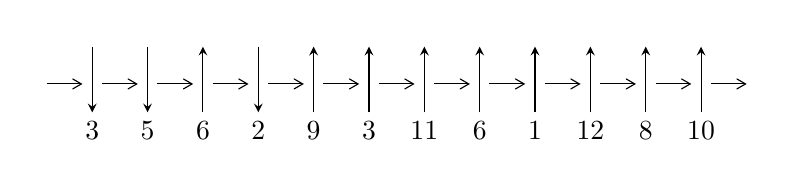
\begin{tikzpicture}[x=20pt, y=17pt]
	% nodes
	\node (C0) at (0, 0) {};
	\node (C1) at (1, 0) {};
	\node (C1U) at (1, +1) {};
	\node (C1D) at (1, -1) {3};

	\node (C2) at (2, 0) {};
	\node (C2U) at (2, +1) {};
	\node (C2D) at (2, -1) {5};

	\node (C3) at (3, 0) {};
	\node (C3U) at (3, +1) {};
	\node (C3D) at (3, -1) {6};

	\node (C4) at (4, 0) {};
	\node (C4U) at (4, +1) {};
	\node (C4D) at (4, -1) {2};

	\node (C5) at (5, 0) {};
	\node (C5U) at (5, +1) {};
	\node (C5D) at (5, -1) {9};

	\node (C6) at (6, 0) {};
	\node (C6U) at (6, +1) {};
	\node (C6D) at (6, -1) {3};

	\node (C7) at (7, 0) {};
	\node (C7U) at (7, +1) {};
	\node (C7D) at (7, -1) {11};

	\node (C8) at (8, 0) {};
	\node (C8U) at (8, +1) {};
	\node (C8D) at (8, -1) {6};

	\node (C9) at (9, 0) {};
	\node (C9U) at (9, +1) {};
	\node (C9D) at (9, -1) {1};

	\node (C10) at (10, 0) {};
	\node (C10U) at (10, +1) {};
	\node (C10D) at (10, -1) {12};

	\node (C11) at (11, 0) {};
	\node (C11U) at (11, +1) {};
	\node (C11D) at (11, -1) {8};

	\node (C12) at (12, 0) {};
	\node (C12U) at (12, +1) {};
	\node (C12D) at (12, -1) {10};
	\node (C13) at (13, 0) {};

	% arrows
	\draw[->,>={angle 60}]
	(C0) edge (C1) (C1) edge (C2) (C2) edge (C3) (C3) edge (C4) (C4) edge (C5) (C5) edge (C6) (C6) edge (C7) (C7) edge (C8) (C8) edge (C9) (C9) edge (C10) (C10) edge (C11) (C11) edge (C12) (C12) edge (C13) ;	\draw[->,>=stealth]
	(C1U) edge (C1D) (C2U) edge (C2D) (C3D) edge (C3U) (C4U) edge (C4D) (C5D) edge (C5U) (C6D) edge (C6U) (C7D) edge (C7U) (C8D) edge (C8U) (C9D) edge (C9U) (C10D) edge (C10U) (C11D) edge (C11U) (C12D) edge (C12U) ;
	\end{tikzpicture} \\
\hhline{~~} \\& 
\textbf{Solving Sequence} \\ \cline{2-2} 
 &
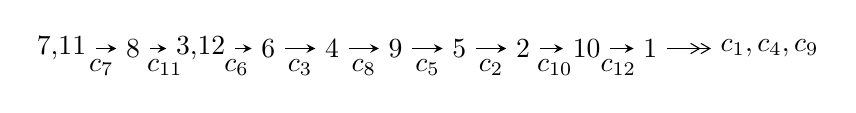
\begin{tikzpicture}[x=23pt, y=7pt]
	% node
	\node (A0) at (-1/8, 0) {7,11};
	\node (A1) at (1, 0) {8};
	\node (A2) at (33/16, 0) {3,12};
	\node (A3) at (25/8, 0) {6};
	\node (A4) at (33/8, 0) {4};
	\node (A5) at (41/8, 0) {9};
	\node (A6) at (49/8, 0) {5};
	\node (A7) at (57/8, 0) {2};
	\node (A8) at (65/8, 0) {10};
	\node (A9) at (73/8, 0) {1};
	\node (C1) at (1/2, -1) {$c_{7}$};
	\node (C2) at (3/2, -1) {$c_{11}$};
	\node (C3) at (21/8, -1) {$c_{6}$};
	\node (C4) at (29/8, -1) {$c_{3}$};
	\node (C5) at (37/8, -1) {$c_{8}$};
	\node (C6) at (45/8, -1) {$c_{5}$};
	\node (C7) at (53/8, -1) {$c_{2}$};
	\node (C8) at (61/8, -1) {$c_{10}$};
	\node (C9) at (69/8, -1) {$c_{12}$};
	\node (A10) at (11, 0) {$c_{1},c_{4},c_{9}$};

	% edge
	\draw[->,>=stealth]	
	(A0) edge (A1) (A1) edge (A2) (A2) edge (A3) (A3) edge (A4) (A4) edge (A5) (A5) edge (A6) (A6) edge (A7) (A7) edge (A8) (A8) edge (A9) ;
	\draw[->>,>={angle 60}]	
	(A9) edge (A10);
\end{tikzpicture} \\ 

\end{tabular} \\

\footnotetext{
The image of knot diagram is generated by the software ``\textbf{Draw programme}" developed by Andrew Bartholomew(\url{http://www.layer8.co.uk/maths/draw/index.htm\#Running-draw}), where we modified some parts for our purpose(\url{https://github.com/CATsTAILs/LinksPainter}).
}\phantom \\ \newline 
\centering \textbf{Ideals for irreducible components\footnotemark of $X_{\text{par}}$} 
 
\begin{align*}
I^u_{1}&=\langle 
-1.55792\times10^{15} u^{51}-2.00897\times10^{15} u^{50}+\cdots+5.52629\times10^{15} b-2.66316\times10^{15},\\
\phantom{I^u_{1}}&\phantom{= \langle  }7.54263\times10^{16} u^{51}+9.53580\times10^{16} u^{50}+\cdots+5.52629\times10^{15} a+1.22505\times10^{17},\;u^{52}+2 u^{51}+\cdots- u+1\rangle \\
I^u_{2}&=\langle 
b,\;-3 u^4- u^3+u^2+a+3 u-4,\;u^5+u^4- u^2+u+1\rangle \\
\\
\end{align*}
\raggedright * 2 irreducible components of $\dim_{\mathbb{C}}=0$, with total 57 representations.\\
\footnotetext{All coefficients of polynomials are rational numbers. But the coefficients are sometimes approximated in decimal forms when there is not enough margin.}
\newpage
\renewcommand{\arraystretch}{1}
\centering \section*{I. $I^u_{1}= \langle -1.56\times10^{15} u^{51}-2.01\times10^{15} u^{50}+\cdots+5.53\times10^{15} b-2.66\times10^{15},\;7.54\times10^{16} u^{51}+9.54\times10^{16} u^{50}+\cdots+5.53\times10^{15} a+1.23\times10^{17},\;u^{52}+2 u^{51}+\cdots- u+1 \rangle$}
\flushleft \textbf{(i) Arc colorings}\\
\begin{tabular}{m{7pt} m{180pt} m{7pt} m{180pt} }
\flushright $a_{7}=$&$\begin{pmatrix}1\\0\end{pmatrix}$ \\
\flushright $a_{11}=$&$\begin{pmatrix}0\\u\end{pmatrix}$ \\
\flushright $a_{8}=$&$\begin{pmatrix}1\\- u^2\end{pmatrix}$ \\
\flushright $a_{3}=$&$\begin{pmatrix}-13.6486 u^{51}-17.2554 u^{50}+\cdots+48.2225 u-22.1677\\0.281910 u^{51}+0.363530 u^{50}+\cdots+0.677139 u+0.481908\end{pmatrix}$ \\
\flushright $a_{12}=$&$\begin{pmatrix}u\\- u^3+u\end{pmatrix}$ \\
\flushright $a_{6}=$&$\begin{pmatrix}3.42922 u^{51}+4.63065 u^{50}+\cdots-12.3515 u+3.71531\\-0.827825 u^{51}-1.65459 u^{50}+\cdots+1.54173 u-0.827822\end{pmatrix}$ \\
\flushright $a_{4}=$&$\begin{pmatrix}-11.4441 u^{51}-15.0654 u^{50}+\cdots+49.3203 u-21.9727\\-2.53719 u^{51}-5.27177 u^{50}+\cdots+4.90575 u-2.33717\end{pmatrix}$ \\
\flushright $a_{9}=$&$\begin{pmatrix}- u^7-2 u^3\\u^9- u^7+3 u^5-2 u^3+u\end{pmatrix}$ \\
\flushright $a_{5}=$&$\begin{pmatrix}2.03316 u^{51}+2.82064 u^{50}+\cdots-9.13837 u+2.51030\\0.154269 u^{51}-0.0905893 u^{50}+\cdots-1.03142 u+0.554276\end{pmatrix}$ \\
\flushright $a_{2}=$&$\begin{pmatrix}-11.7150 u^{51}-14.8966 u^{50}+\cdots+44.4993 u-21.1883\\-1.02663 u^{51}-2.45529 u^{50}+\cdots+2.73997 u-0.626644\end{pmatrix}$ \\
\flushright $a_{10}=$&$\begin{pmatrix}- u^3\\u^5- u^3+u\end{pmatrix}$ \\
\flushright $a_{1}=$&$\begin{pmatrix}u^5+u\\- u^7+u^5-2 u^3+u\end{pmatrix}$\\&\end{tabular}
\flushleft \textbf{(ii) Obstruction class $= -1$}\\~\\
\flushleft \textbf{(iii) Cusp Shapes $= -\frac{820656989676521272}{5526285094326109} u^{51}-\frac{1059949487703439182}{5526285094326109} u^{50}+\cdots+\frac{2787762104200863436}{5526285094326109} u-\frac{1166602438311091155}{5526285094326109}$}\\~\\
\newpage\renewcommand{\arraystretch}{1}
\flushleft \textbf{(iv) u-Polynomials at the component}\newline \\
\begin{tabular}{m{50pt}|m{274pt}}
Crossings & \hspace{64pt}u-Polynomials at each crossing \\
\hline $$\begin{aligned}c_{1}\end{aligned}$$&$\begin{aligned}
&u^{52}+22 u^{51}+\cdots+621 u+1
\end{aligned}$\\
\hline $$\begin{aligned}c_{2},c_{4}\end{aligned}$$&$\begin{aligned}
&u^{52}-6 u^{51}+\cdots+33 u-1
\end{aligned}$\\
\hline $$\begin{aligned}c_{3},c_{6}\end{aligned}$$&$\begin{aligned}
&u^{52}+7 u^{51}+\cdots-1000 u^2+32
\end{aligned}$\\
\hline $$\begin{aligned}c_{5},c_{8}\end{aligned}$$&$\begin{aligned}
&u^{52}+2 u^{51}+\cdots- u-1
\end{aligned}$\\
\hline $$\begin{aligned}c_{7},c_{11}\end{aligned}$$&$\begin{aligned}
&u^{52}-2 u^{51}+\cdots+u+1
\end{aligned}$\\
\hline $$\begin{aligned}c_{9},c_{10},c_{12}\end{aligned}$$&$\begin{aligned}
&u^{52}-14 u^{51}+\cdots-3 u+1
\end{aligned}$\\
\hline
\end{tabular}\\~\\
\newpage\renewcommand{\arraystretch}{1}
\flushleft \textbf{(v) Riley Polynomials at the component}\newline \\
\begin{tabular}{m{50pt}|m{274pt}}
Crossings & \hspace{64pt}Riley Polynomials at each crossing \\
\hline $$\begin{aligned}c_{1}\end{aligned}$$&$\begin{aligned}
&y^{52}+22 y^{51}+\cdots-353149 y+1
\end{aligned}$\\
\hline $$\begin{aligned}c_{2},c_{4}\end{aligned}$$&$\begin{aligned}
&y^{52}-22 y^{51}+\cdots-621 y+1
\end{aligned}$\\
\hline $$\begin{aligned}c_{3},c_{6}\end{aligned}$$&$\begin{aligned}
&y^{52}-33 y^{51}+\cdots-64000 y+1024
\end{aligned}$\\
\hline $$\begin{aligned}c_{5},c_{8}\end{aligned}$$&$\begin{aligned}
&y^{52}+14 y^{51}+\cdots-3 y+1
\end{aligned}$\\
\hline $$\begin{aligned}c_{7},c_{11}\end{aligned}$$&$\begin{aligned}
&y^{52}-14 y^{51}+\cdots-3 y+1
\end{aligned}$\\
\hline $$\begin{aligned}c_{9},c_{10},c_{12}\end{aligned}$$&$\begin{aligned}
&y^{52}+50 y^{51}+\cdots-3 y+1
\end{aligned}$\\
\hline
\end{tabular}\\~\\
\newpage\flushleft \textbf{(vi) Complex Volumes and Cusp Shapes}
$$\begin{array}{c|c|c}  
\text{Solutions to }I^u_{1}& \I (\text{vol} + \sqrt{-1}CS) & \text{Cusp shape}\\
 \hline 
\begin{aligned}
u &= \phantom{-}1.016700 + 0.228557 I \\
a &= \phantom{-}2.72812 - 0.43036 I \\
b &= -1.51670 - 0.32511 I\end{aligned}
 & \phantom{-}6.00023 + 3.38638 I & \phantom{-}10.71662 - 4.19927 I \\ \hline\begin{aligned}
u &= \phantom{-}1.016700 - 0.228557 I \\
a &= \phantom{-}2.72812 + 0.43036 I \\
b &= -1.51670 + 0.32511 I\end{aligned}
 & \phantom{-}6.00023 - 3.38638 I & \phantom{-}10.71662 + 4.19927 I \\ \hline\begin{aligned}
u &= \phantom{-}0.823924 + 0.656561 I \\
a &= -0.484808 + 0.298032 I \\
b &= \phantom{-}0.495386 - 0.141113 I\end{aligned}
 & -2.12988 + 2.49537 I & \phantom{-}6.00000 - 4.33112 I \\ \hline\begin{aligned}
u &= \phantom{-}0.823924 - 0.656561 I \\
a &= -0.484808 - 0.298032 I \\
b &= \phantom{-}0.495386 + 0.141113 I\end{aligned}
 & -2.12988 - 2.49537 I & \phantom{-}6.00000 + 4.33112 I \\ \hline\begin{aligned}
u &= \phantom{-}0.671451 + 0.825112 I \\
a &= -0.172842 + 0.134029 I \\
b &= \phantom{-}0.986460 + 0.139928 I\end{aligned}
 & -1.94375 + 3.12402 I & \phantom{-}6.00000 - 5.50076 I \\ \hline\begin{aligned}
u &= \phantom{-}0.671451 - 0.825112 I \\
a &= -0.172842 - 0.134029 I \\
b &= \phantom{-}0.986460 - 0.139928 I\end{aligned}
 & -1.94375 - 3.12402 I & \phantom{-}6.00000 + 5.50076 I \\ \hline\begin{aligned}
u &= -1.019540 + 0.324660 I \\
a &= \phantom{-}1.95326 + 1.46461 I \\
b &= -1.375970 + 0.072193 I\end{aligned}
 & \phantom{-}5.42581 - 2.84612 I & \phantom{-}6.00000 + 4.09308 I \\ \hline\begin{aligned}
u &= -1.019540 - 0.324660 I \\
a &= \phantom{-}1.95326 - 1.46461 I \\
b &= -1.375970 - 0.072193 I\end{aligned}
 & \phantom{-}5.42581 + 2.84612 I & \phantom{-}6.00000 - 4.09308 I \\ \hline\begin{aligned}
u &= -1.067180 + 0.215417 I \\
a &= -2.01848 - 1.25744 I \\
b &= \phantom{-}1.328520 + 0.303236 I\end{aligned}
 & \phantom{-}4.97698 + 2.99566 I & \phantom{-0.000000 } 0 \\ \hline\begin{aligned}
u &= -1.067180 - 0.215417 I \\
a &= -2.01848 + 1.25744 I \\
b &= \phantom{-}1.328520 - 0.303236 I\end{aligned}
 & \phantom{-}4.97698 - 2.99566 I & \phantom{-0.000000 } 0\\
 \hline 
 \end{array}$$\newpage$$\begin{array}{c|c|c}  
\text{Solutions to }I^u_{1}& \I (\text{vol} + \sqrt{-1}CS) & \text{Cusp shape}\\
 \hline 
\begin{aligned}
u &= \phantom{-}1.061390 + 0.321917 I \\
a &= -2.57122 + 0.55153 I \\
b &= \phantom{-}1.41215 + 0.59209 I\end{aligned}
 & \phantom{-}4.33370 + 9.78968 I & \phantom{-0.000000 } 0 \\ \hline\begin{aligned}
u &= \phantom{-}1.061390 - 0.321917 I \\
a &= -2.57122 - 0.55153 I \\
b &= \phantom{-}1.41215 - 0.59209 I\end{aligned}
 & \phantom{-}4.33370 - 9.78968 I & \phantom{-0.000000 } 0 \\ \hline\begin{aligned}
u &= -0.763594 + 0.816084 I \\
a &= -0.008414 + 0.288534 I \\
b &= -1.43047 - 0.79666 I\end{aligned}
 & -0.81354 + 2.41917 I & \phantom{-0.000000 } 0 \\ \hline\begin{aligned}
u &= -0.763594 - 0.816084 I \\
a &= -0.008414 - 0.288534 I \\
b &= -1.43047 + 0.79666 I\end{aligned}
 & -0.81354 - 2.41917 I & \phantom{-0.000000 } 0 \\ \hline\begin{aligned}
u &= \phantom{-}0.829935 + 0.258628 I \\
a &= \phantom{-}0.589363 + 1.277800 I \\
b &= -0.015897 - 1.194290 I\end{aligned}
 & -0.05696 + 3.40025 I & \phantom{-}6.00000 - 9.58209 I \\ \hline\begin{aligned}
u &= \phantom{-}0.829935 - 0.258628 I \\
a &= \phantom{-}0.589363 - 1.277800 I \\
b &= -0.015897 + 1.194290 I\end{aligned}
 & -0.05696 - 3.40025 I & \phantom{-}6.00000 + 9.58209 I \\ \hline\begin{aligned}
u &= \phantom{-}0.856907 + 0.769828 I \\
a &= \phantom{-}0.98921 - 2.18567 I \\
b &= -0.330878 - 0.523016 I\end{aligned}
 & -4.80216 + 2.18470 I & \phantom{-0.000000 } 0 \\ \hline\begin{aligned}
u &= \phantom{-}0.856907 - 0.769828 I \\
a &= \phantom{-}0.98921 + 2.18567 I \\
b &= -0.330878 + 0.523016 I\end{aligned}
 & -4.80216 - 2.18470 I & \phantom{-0.000000 } 0 \\ \hline\begin{aligned}
u &= -0.843215 + 0.806418 I \\
a &= -1.119580 - 0.651664 I \\
b &= \phantom{-}0.55289 - 1.60337 I\end{aligned}
 & -6.35990 + 0.70710 I & \phantom{-0.000000 } 0 \\ \hline\begin{aligned}
u &= -0.843215 - 0.806418 I \\
a &= -1.119580 + 0.651664 I \\
b &= \phantom{-}0.55289 + 1.60337 I\end{aligned}
 & -6.35990 - 0.70710 I & \phantom{-0.000000 } 0\\
 \hline 
 \end{array}$$\newpage$$\begin{array}{c|c|c}  
\text{Solutions to }I^u_{1}& \I (\text{vol} + \sqrt{-1}CS) & \text{Cusp shape}\\
 \hline 
\begin{aligned}
u &= -0.815699 + 0.149945 I \\
a &= -1.65430 - 0.16657 I \\
b &= -0.000259 - 0.620302 I\end{aligned}
 & \phantom{-}0.447505 - 0.352674 I & \phantom{-}7.09954 + 0.50809 I \\ \hline\begin{aligned}
u &= -0.815699 - 0.149945 I \\
a &= -1.65430 + 0.16657 I \\
b &= -0.000259 + 0.620302 I\end{aligned}
 & \phantom{-}0.447505 + 0.352674 I & \phantom{-}7.09954 - 0.50809 I \\ \hline\begin{aligned}
u &= -0.770843 + 0.892832 I \\
a &= -0.1123930 + 0.0783246 I \\
b &= \phantom{-}1.32848 + 0.83591 I\end{aligned}
 & -3.73354 + 8.81773 I & \phantom{-0.000000 } 0 \\ \hline\begin{aligned}
u &= -0.770843 - 0.892832 I \\
a &= -0.1123930 - 0.0783246 I \\
b &= \phantom{-}1.32848 - 0.83591 I\end{aligned}
 & -3.73354 - 8.81773 I & \phantom{-0.000000 } 0 \\ \hline\begin{aligned}
u &= \phantom{-}0.906595 + 0.760633 I \\
a &= -0.23718 + 1.51693 I \\
b &= -0.277122 + 0.612791 I\end{aligned}
 & -4.64898 + 3.59909 I & \phantom{-0.000000 } 0 \\ \hline\begin{aligned}
u &= \phantom{-}0.906595 - 0.760633 I \\
a &= -0.23718 - 1.51693 I \\
b &= -0.277122 - 0.612791 I\end{aligned}
 & -4.64898 - 3.59909 I & \phantom{-0.000000 } 0 \\ \hline\begin{aligned}
u &= \phantom{-}0.797815 + 0.885175 I \\
a &= -0.096669 + 0.136453 I \\
b &= -1.090370 + 0.347341 I\end{aligned}
 & -2.52853 - 1.37505 I & \phantom{-0.000000 } 0 \\ \hline\begin{aligned}
u &= \phantom{-}0.797815 - 0.885175 I \\
a &= -0.096669 - 0.136453 I \\
b &= -1.090370 - 0.347341 I\end{aligned}
 & -2.52853 + 1.37505 I & \phantom{-0.000000 } 0 \\ \hline\begin{aligned}
u &= -0.889829 + 0.799881 I \\
a &= -0.98021 - 1.11750 I \\
b &= \phantom{-}1.70487 + 0.08098 I\end{aligned}
 & -7.98633 - 2.99814 I & \phantom{-0.000000 } 0 \\ \hline\begin{aligned}
u &= -0.889829 - 0.799881 I \\
a &= -0.98021 + 1.11750 I \\
b &= \phantom{-}1.70487 - 0.08098 I\end{aligned}
 & -7.98633 + 2.99814 I & \phantom{-0.000000 } 0\\
 \hline 
 \end{array}$$\newpage$$\begin{array}{c|c|c}  
\text{Solutions to }I^u_{1}& \I (\text{vol} + \sqrt{-1}CS) & \text{Cusp shape}\\
 \hline 
\begin{aligned}
u &= -0.929422 + 0.783147 I \\
a &= \phantom{-}1.103730 - 0.206306 I \\
b &= \phantom{-}0.41722 + 1.67850 I\end{aligned}
 & -6.09427 - 6.67098 I & \phantom{-0.000000 } 0 \\ \hline\begin{aligned}
u &= -0.929422 - 0.783147 I \\
a &= \phantom{-}1.103730 + 0.206306 I \\
b &= \phantom{-}0.41722 - 1.67850 I\end{aligned}
 & -6.09427 + 6.67098 I & \phantom{-0.000000 } 0 \\ \hline\begin{aligned}
u &= \phantom{-}1.003030 + 0.726539 I \\
a &= -0.665678 + 1.244470 I \\
b &= \phantom{-}1.095740 + 0.014542 I\end{aligned}
 & -0.95751 + 2.64231 I & \phantom{-0.000000 } 0 \\ \hline\begin{aligned}
u &= \phantom{-}1.003030 - 0.726539 I \\
a &= -0.665678 - 1.244470 I \\
b &= \phantom{-}1.095740 - 0.014542 I\end{aligned}
 & -0.95751 - 2.64231 I & \phantom{-0.000000 } 0 \\ \hline\begin{aligned}
u &= \phantom{-}0.083300 + 0.756806 I \\
a &= -0.131209 - 0.090120 I \\
b &= \phantom{-}1.241510 - 0.510914 I\end{aligned}
 & \phantom{-}1.11117 - 6.07445 I & \phantom{-}2.28728 + 4.99398 I \\ \hline\begin{aligned}
u &= \phantom{-}0.083300 - 0.756806 I \\
a &= -0.131209 + 0.090120 I \\
b &= \phantom{-}1.241510 + 0.510914 I\end{aligned}
 & \phantom{-}1.11117 + 6.07445 I & \phantom{-}2.28728 - 4.99398 I \\ \hline\begin{aligned}
u &= -0.980620 + 0.759025 I \\
a &= \phantom{-}1.48052 + 1.47301 I \\
b &= -1.57827 + 0.76747 I\end{aligned}
 & -0.15374 - 8.33088 I & \phantom{-0.000000 } 0 \\ \hline\begin{aligned}
u &= -0.980620 - 0.759025 I \\
a &= \phantom{-}1.48052 - 1.47301 I \\
b &= -1.57827 - 0.76747 I\end{aligned}
 & -0.15374 + 8.33088 I & \phantom{-0.000000 } 0 \\ \hline\begin{aligned}
u &= \phantom{-}0.996725 + 0.804943 I \\
a &= \phantom{-}0.69605 - 1.42479 I \\
b &= -1.168190 - 0.406129 I\end{aligned}
 & -1.90172 + 7.64393 I & \phantom{-0.000000 } 0 \\ \hline\begin{aligned}
u &= \phantom{-}0.996725 - 0.804943 I \\
a &= \phantom{-}0.69605 + 1.42479 I \\
b &= -1.168190 + 0.406129 I\end{aligned}
 & -1.90172 - 7.64393 I & \phantom{-0.000000 } 0\\
 \hline 
 \end{array}$$\newpage$$\begin{array}{c|c|c}  
\text{Solutions to }I^u_{1}& \I (\text{vol} + \sqrt{-1}CS) & \text{Cusp shape}\\
 \hline 
\begin{aligned}
u &= -1.011220 + 0.795658 I \\
a &= -1.51176 - 1.46953 I \\
b &= \phantom{-}1.39466 - 0.85421 I\end{aligned}
 & -2.9794 - 15.0713 I & \phantom{-0.000000 } 0 \\ \hline\begin{aligned}
u &= -1.011220 - 0.795658 I \\
a &= -1.51176 + 1.46953 I \\
b &= \phantom{-}1.39466 + 0.85421 I\end{aligned}
 & -2.9794 + 15.0713 I & \phantom{-0.000000 } 0 \\ \hline\begin{aligned}
u &= -0.698273\phantom{ +0.000000I} \\
a &= \phantom{-}8.42855\phantom{ +0.000000I} \\
b &= -0.206931\phantom{ +0.000000I}\end{aligned}
 & -0.693373\phantom{ +0.000000I} & \phantom{-}108.630\phantom{ +0.000000I} \\ \hline\begin{aligned}
u &= -0.939941 + 0.914479 I \\
a &= \phantom{-}0.055763 - 0.275557 I \\
b &= \phantom{-}0.491327 - 0.017560 I\end{aligned}
 & -12.27210 - 3.36480 I & \phantom{-0.000000 } 0 \\ \hline\begin{aligned}
u &= -0.939941 - 0.914479 I \\
a &= \phantom{-}0.055763 + 0.275557 I \\
b &= \phantom{-}0.491327 + 0.017560 I\end{aligned}
 & -12.27210 + 3.36480 I & \phantom{-0.000000 } 0 \\ \hline\begin{aligned}
u &= -0.095263 + 0.656941 I \\
a &= -0.107033 - 0.214568 I \\
b &= -1.209340 + 0.178713 I\end{aligned}
 & \phantom{-}2.53391 - 0.61006 I & \phantom{-}4.82513 + 0.42624 I \\ \hline\begin{aligned}
u &= -0.095263 - 0.656941 I \\
a &= -0.107033 + 0.214568 I \\
b &= -1.209340 - 0.178713 I\end{aligned}
 & \phantom{-}2.53391 + 0.61006 I & \phantom{-}4.82513 - 0.42624 I \\ \hline\begin{aligned}
u &= \phantom{-}0.581935 + 0.257196 I \\
a &= -2.52005 + 0.53236 I \\
b &= \phantom{-}0.898782 - 0.422027 I\end{aligned}
 & -2.37470 + 1.17859 I & -0.43614 - 4.23765 I \\ \hline\begin{aligned}
u &= \phantom{-}0.581935 - 0.257196 I \\
a &= -2.52005 - 0.53236 I \\
b &= \phantom{-}0.898782 + 0.422027 I\end{aligned}
 & -2.37470 - 1.17859 I & -0.43614 + 4.23765 I \\ \hline\begin{aligned}
u &= -0.607842\phantom{ +0.000000I} \\
a &= -0.654513\phantom{ +0.000000I} \\
b &= -0.202346\phantom{ +0.000000I}\end{aligned}
 & \phantom{-}0.846925\phantom{ +0.000000I} & \phantom{-}12.0260\phantom{ +0.000000I}\\
 \hline 
 \end{array}$$\newpage$$\begin{array}{c|c|c}  
\text{Solutions to }I^u_{1}& \I (\text{vol} + \sqrt{-1}CS) & \text{Cusp shape}\\
 \hline 
\begin{aligned}
u &= \phantom{-}0.149713 + 0.331460 I \\
a &= -2.09121 + 1.21238 I \\
b &= \phantom{-}0.350124 + 0.778422 I\end{aligned}
 & -1.82510 - 1.05647 I & -2.50964 + 1.48510 I \\ \hline\begin{aligned}
u &= \phantom{-}0.149713 - 0.331460 I \\
a &= -2.09121 - 1.21238 I \\
b &= \phantom{-}0.350124 - 0.778422 I\end{aligned}
 & -1.82510 + 1.05647 I & -2.50964 - 1.48510 I\\
 \hline 
 \end{array}$$\newpage\newpage\renewcommand{\arraystretch}{1}
\centering \section*{II. $I^u_{2}= \langle b,\;-3 u^4- u^3+u^2+a+3 u-4,\;u^5+u^4- u^2+u+1 \rangle$}
\flushleft \textbf{(i) Arc colorings}\\
\begin{tabular}{m{7pt} m{180pt} m{7pt} m{180pt} }
\flushright $a_{7}=$&$\begin{pmatrix}1\\0\end{pmatrix}$ \\
\flushright $a_{11}=$&$\begin{pmatrix}0\\u\end{pmatrix}$ \\
\flushright $a_{8}=$&$\begin{pmatrix}1\\- u^2\end{pmatrix}$ \\
\flushright $a_{3}=$&$\begin{pmatrix}3 u^4+u^3- u^2-3 u+4\\0\end{pmatrix}$ \\
\flushright $a_{12}=$&$\begin{pmatrix}u\\- u^3+u\end{pmatrix}$ \\
\flushright $a_{6}=$&$\begin{pmatrix}1\\0\end{pmatrix}$ \\
\flushright $a_{4}=$&$\begin{pmatrix}3 u^4+u^3- u^2-3 u+4\\0\end{pmatrix}$ \\
\flushright $a_{9}=$&$\begin{pmatrix}- u^2+1\\- u^2\end{pmatrix}$ \\
\flushright $a_{5}=$&$\begin{pmatrix}u^4- u^2+1\\u^4\end{pmatrix}$ \\
\flushright $a_{2}=$&$\begin{pmatrix}2 u^4+u^3-3 u+3\\- u^4\end{pmatrix}$ \\
\flushright $a_{10}=$&$\begin{pmatrix}- u^3\\- u^4- u^3+u^2-1\end{pmatrix}$ \\
\flushright $a_{1}=$&$\begin{pmatrix}- u^4+u^2-1\\- u^4\end{pmatrix}$\\&\end{tabular}
\flushleft \textbf{(ii) Obstruction class $= 1$}\\~\\
\flushleft \textbf{(iii) Cusp Shapes $= -10 u^4-7 u^3- u^2+10 u-19$}\\~\\
\newpage\renewcommand{\arraystretch}{1}
\flushleft \textbf{(iv) u-Polynomials at the component}\newline \\
\begin{tabular}{m{50pt}|m{274pt}}
Crossings & \hspace{64pt}u-Polynomials at each crossing \\
\hline $$\begin{aligned}c_{1},c_{2}\end{aligned}$$&$\begin{aligned}
&(u-1)^5
\end{aligned}$\\
\hline $$\begin{aligned}c_{3},c_{6}\end{aligned}$$&$\begin{aligned}
&u^5
\end{aligned}$\\
\hline $$\begin{aligned}c_{4}\end{aligned}$$&$\begin{aligned}
&(u+1)^5
\end{aligned}$\\
\hline $$\begin{aligned}c_{5},c_{9},c_{10}\end{aligned}$$&$\begin{aligned}
&u^5+u^4+4 u^3+3 u^2+3 u+1
\end{aligned}$\\
\hline $$\begin{aligned}c_{7}\end{aligned}$$&$\begin{aligned}
&u^5+u^4- u^2+u+1
\end{aligned}$\\
\hline $$\begin{aligned}c_{8},c_{12}\end{aligned}$$&$\begin{aligned}
&u^5- u^4+4 u^3-3 u^2+3 u-1
\end{aligned}$\\
\hline $$\begin{aligned}c_{11}\end{aligned}$$&$\begin{aligned}
&u^5- u^4+u^2+u-1
\end{aligned}$\\
\hline
\end{tabular}\\~\\
\newpage\renewcommand{\arraystretch}{1}
\flushleft \textbf{(v) Riley Polynomials at the component}\newline \\
\begin{tabular}{m{50pt}|m{274pt}}
Crossings & \hspace{64pt}Riley Polynomials at each crossing \\
\hline $$\begin{aligned}c_{1},c_{2},c_{4}\end{aligned}$$&$\begin{aligned}
&(y-1)^5
\end{aligned}$\\
\hline $$\begin{aligned}c_{3},c_{6}\end{aligned}$$&$\begin{aligned}
&y^5
\end{aligned}$\\
\hline $$\begin{aligned}c_{5},c_{8},c_{9}\\c_{10},c_{12}\end{aligned}$$&$\begin{aligned}
&y^5+7 y^4+16 y^3+13 y^2+3 y-1
\end{aligned}$\\
\hline $$\begin{aligned}c_{7},c_{11}\end{aligned}$$&$\begin{aligned}
&y^5- y^4+4 y^3-3 y^2+3 y-1
\end{aligned}$\\
\hline
\end{tabular}\\~\\
\newpage\flushleft \textbf{(vi) Complex Volumes and Cusp Shapes}
$$\begin{array}{c|c|c}  
\text{Solutions to }I^u_{2}& \I (\text{vol} + \sqrt{-1}CS) & \text{Cusp shape}\\
 \hline 
\begin{aligned}
u &= \phantom{-}0.758138 + 0.584034 I \\
a &= -1.036940 - 0.588205 I \\
b &= \phantom{-0.000000 } 0\end{aligned}
 & -3.46474 + 2.21397 I & -1.97599 - 4.83884 I \\ \hline\begin{aligned}
u &= \phantom{-}0.758138 - 0.584034 I \\
a &= -1.036940 + 0.588205 I \\
b &= \phantom{-0.000000 } 0\end{aligned}
 & -3.46474 - 2.21397 I & -1.97599 + 4.83884 I \\ \hline\begin{aligned}
u &= -0.935538 + 0.903908 I \\
a &= -0.348360 + 0.023996 I \\
b &= \phantom{-0.000000 } 0\end{aligned}
 & -12.60320 - 3.33174 I & -10.16346 + 1.25445 I \\ \hline\begin{aligned}
u &= -0.935538 - 0.903908 I \\
a &= -0.348360 - 0.023996 I \\
b &= \phantom{-0.000000 } 0\end{aligned}
 & -12.60320 + 3.33174 I & -10.16346 - 1.25445 I \\ \hline\begin{aligned}
u &= -0.645200\phantom{ +0.000000I} \\
a &= \phantom{-}5.77061\phantom{ +0.000000I} \\
b &= \phantom{-0.000000 } 0\end{aligned}
 & -0.762751\phantom{ +0.000000I} & -25.7210\phantom{ +0.000000I}\\
 \hline 
 \end{array}$$\newpage
\newpage\renewcommand{\arraystretch}{1}
\centering \section*{ III. u-Polynomials}
\begin{tabular}{m{50pt}|m{274pt}}
Crossings & \hspace{64pt}u-Polynomials at each crossing \\
\hline $$\begin{aligned}c_{1}\end{aligned}$$&$\begin{aligned}
&((u-1)^5)(u^{52}+22 u^{51}+\cdots+621 u+1)
\end{aligned}$\\
\hline $$\begin{aligned}c_{2}\end{aligned}$$&$\begin{aligned}
&((u-1)^5)(u^{52}-6 u^{51}+\cdots+33 u-1)
\end{aligned}$\\
\hline $$\begin{aligned}c_{3},c_{6}\end{aligned}$$&$\begin{aligned}
&u^5(u^{52}+7 u^{51}+\cdots-1000 u^2+32)
\end{aligned}$\\
\hline $$\begin{aligned}c_{4}\end{aligned}$$&$\begin{aligned}
&((u+1)^5)(u^{52}-6 u^{51}+\cdots+33 u-1)
\end{aligned}$\\
\hline $$\begin{aligned}c_{5}\end{aligned}$$&$\begin{aligned}
&(u^5+u^4+4 u^3+3 u^2+3 u+1)(u^{52}+2 u^{51}+\cdots- u-1)
\end{aligned}$\\
\hline $$\begin{aligned}c_{7}\end{aligned}$$&$\begin{aligned}
&(u^5+u^4- u^2+u+1)(u^{52}-2 u^{51}+\cdots+u+1)
\end{aligned}$\\
\hline $$\begin{aligned}c_{8}\end{aligned}$$&$\begin{aligned}
&(u^5- u^4+4 u^3-3 u^2+3 u-1)(u^{52}+2 u^{51}+\cdots- u-1)
\end{aligned}$\\
\hline $$\begin{aligned}c_{9},c_{10}\end{aligned}$$&$\begin{aligned}
&(u^5+u^4+4 u^3+3 u^2+3 u+1)(u^{52}-14 u^{51}+\cdots-3 u+1)
\end{aligned}$\\
\hline $$\begin{aligned}c_{11}\end{aligned}$$&$\begin{aligned}
&(u^5- u^4+u^2+u-1)(u^{52}-2 u^{51}+\cdots+u+1)
\end{aligned}$\\
\hline $$\begin{aligned}c_{12}\end{aligned}$$&$\begin{aligned}
&(u^5- u^4+4 u^3-3 u^2+3 u-1)(u^{52}-14 u^{51}+\cdots-3 u+1)
\end{aligned}$\\
\hline
\end{tabular}\newpage\renewcommand{\arraystretch}{1}
\centering \section*{ IV. Riley Polynomials}
\begin{tabular}{m{50pt}|m{274pt}}
Crossings & \hspace{64pt}Riley Polynomials at each crossing \\
\hline $$\begin{aligned}c_{1}\end{aligned}$$&$\begin{aligned}
&((y-1)^5)(y^{52}+22 y^{51}+\cdots-353149 y+1)
\end{aligned}$\\
\hline $$\begin{aligned}c_{2},c_{4}\end{aligned}$$&$\begin{aligned}
&((y-1)^5)(y^{52}-22 y^{51}+\cdots-621 y+1)
\end{aligned}$\\
\hline $$\begin{aligned}c_{3},c_{6}\end{aligned}$$&$\begin{aligned}
&y^5(y^{52}-33 y^{51}+\cdots-64000 y+1024)
\end{aligned}$\\
\hline $$\begin{aligned}c_{5},c_{8}\end{aligned}$$&$\begin{aligned}
&(y^5+7 y^4+16 y^3+13 y^2+3 y-1)(y^{52}+14 y^{51}+\cdots-3 y+1)
\end{aligned}$\\
\hline $$\begin{aligned}c_{7},c_{11}\end{aligned}$$&$\begin{aligned}
&(y^5- y^4+4 y^3-3 y^2+3 y-1)(y^{52}-14 y^{51}+\cdots-3 y+1)
\end{aligned}$\\
\hline $$\begin{aligned}c_{9},c_{10},c_{12}\end{aligned}$$&$\begin{aligned}
&(y^5+7 y^4+16 y^3+13 y^2+3 y-1)(y^{52}+50 y^{51}+\cdots-3 y+1)
\end{aligned}$\\
\hline
\end{tabular}
\vskip 2pc
\end{document}